
	\chapter{Simple dependency -sd}
	Let assume that there is a fact such that, there is only one action producing this fact and only one action deleting this fact (there is no action that has got this fact in prevail precondition). Then it may seem reasonable to merge both actions to only one instead to lower number of actions. 
	
	This operation does such a merging of actions, but the thing is not so trivial as it may seem. To merge both actions they have to be \emph{atomic}. In short it means that if action adding the fact is applied, then the second action can be applied as well. 
	
	\begin{figure}
		\begin{subfigure}[b]{0.4\textwidth}
			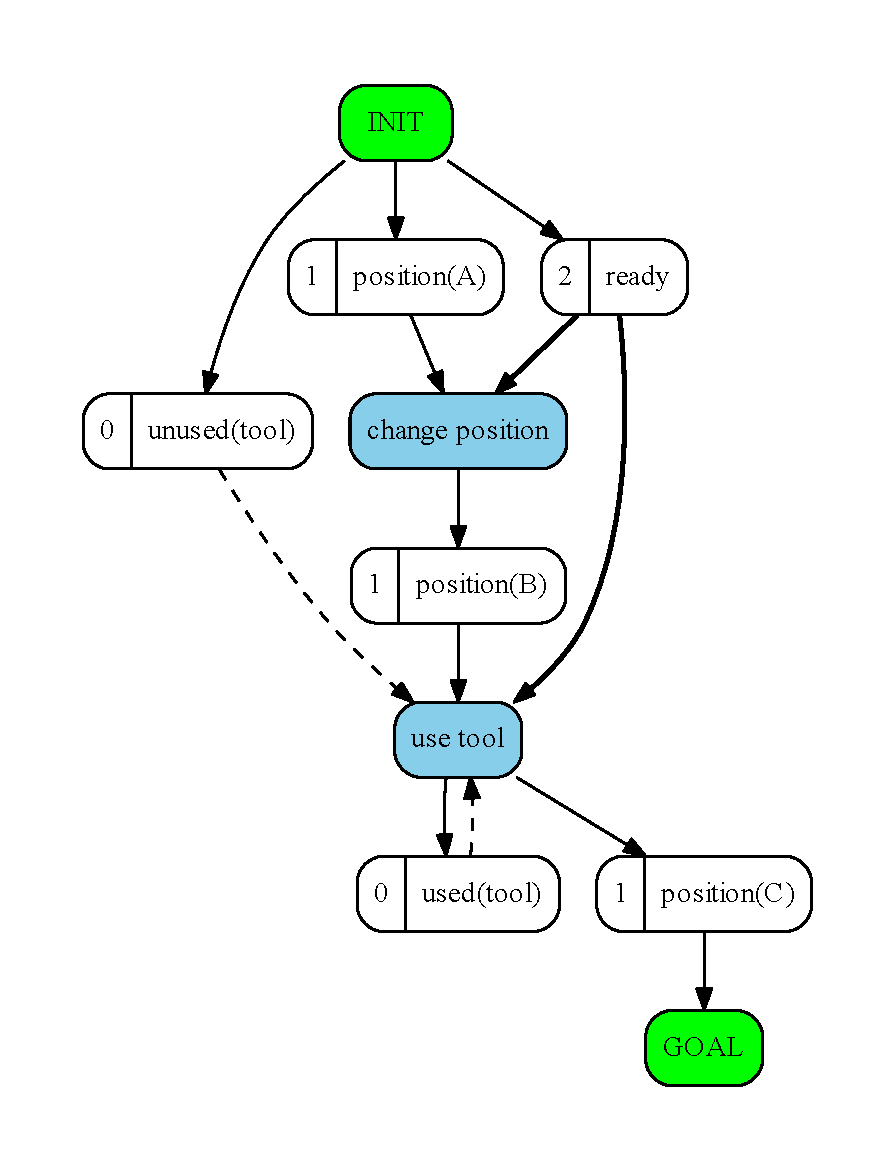
\includegraphics[scale=0.4]{simpleDependency/figures/simple_input}
			\caption{before reduction}
		\end{subfigure}	
		\begin{subfigure}[b]{0.4\textwidth}
			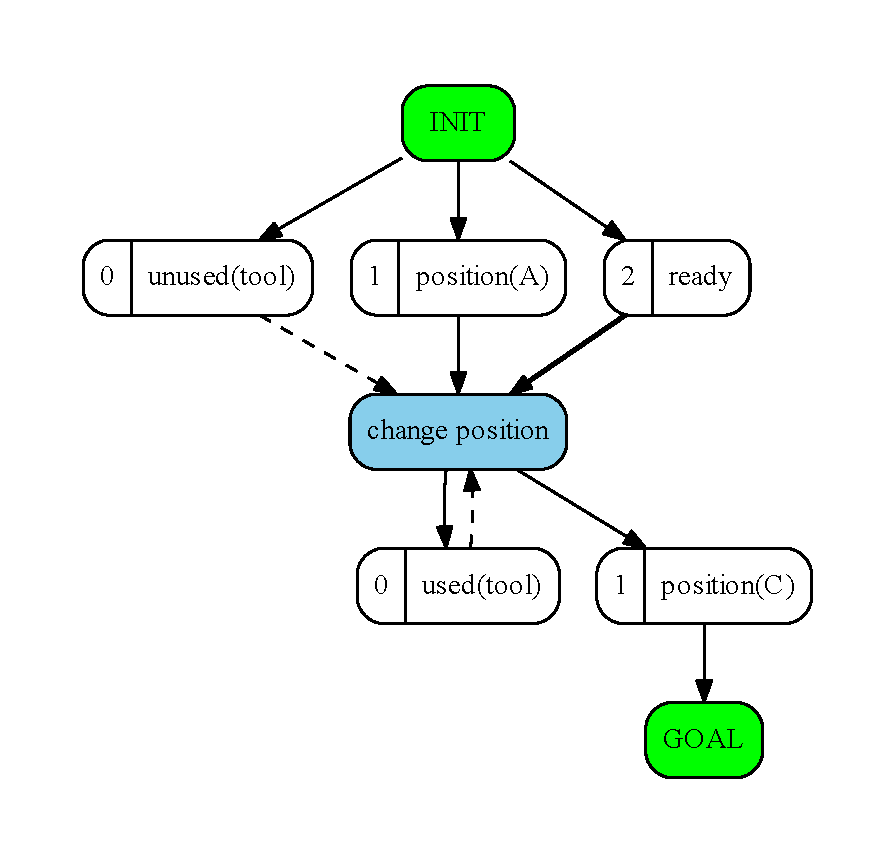
\includegraphics[scale=0.4]{simpleDependency/figures/simple_output}
			\caption{after reduction}
		\end{subfigure}
		\caption{actions \emph{change position} and \emph{use tool} can be merged to one}		
	\end{figure}
	
	\section{Reduce operation}
	Lets have SAS in form $<\vars, \init, \goal, \actions, \mutexes{}>$. This operation will be executed if the following will hold:
	
	\begin{enumerate}
		\item there is a value $u$, which is not in init and not in goal; $u \notin \init$, $u \notin \goal$
		\item only one action $a_i$ that adds $u$; $|\{a | a \in \actions, u \in \add{a}\}| = 1$
		\item $a_i$ adds only $u$; $\add{a_i} = \{u\}$
		\item only one action $a_j$ that needs $u$; $|\{a | a \in \actions, u \in \pre{a} \lor u \in \del{a} \}| = 1$
		\item to ensure atomicity there must hold that $\pre{a_i} \subseteq \pre{a_j}$
		\item if there is a effect in $\eff{a_j}$ of type $<-1,w>$, then any value of $\var{w}$ must not be in $\pre{a_i}$
	\end{enumerate}
	
	We assume that if a value is in $del$ of a operator, then the value is not present in the operator's $pre$. Now, the reduction is following:
	
	\begin{enumerate}
		\item $\dom{v} := \dom{v} \setminus \{u\}$ 
		\item $u$ is also removed from mutexes as in -dv; final mutexes are stored to $\mutexes{}'$
		\item if $u \in \pre{a_j}$ then $p \leftarrow (\pre{a_i} \cup \pre{a_j}) \setminus \{u\}$, $e \leftarrow <\del{a_i} \cup \del{a_j}, \add{a_i} \cup \add{a_j}>$ \label{SD:out:wrong}
		\item if $u \in \del{a_j}$ then set $u_p : <u_p, u> \in \eff{a_i}, u_n : <u, u_n> \in \eff{a_j}$ $p \leftarrow \pre{a_i} \cup \pre{a_j}$, $e \leftarrow <(\del{a_i} \cup \del{a_j}) \setminus \{u\}, (\add{a_i} \cup \add{a_j}) \setminus \{u\}>$, so instead of two effect $<u_p, u>, <u, u_n>$ there is only one $<u_p, u_n>$ \label{SD:out:inEffect}
		\item $a_n \leftarrow <p,e>$
		\item $\actions{}' \leftarrow (\actions \setminus \{a_i, a_j\}) \cup \{a_n\}$		
	\end{enumerate}
	
	Output of the reduction is SAS $<\vars{}, \init{}, \goal{}, \actions{}', \mutexes{}'>$.
	
	
	\textbf{There is a mistake:} this procedure is implemented in the code but it does not follow the difference of $u$ being in prevail precondition and delete of an action right. If $u$ is in delete effect of $a_j$, then it will work fine. But if $u$ is in prevail precondition of $a_j$, then by merging $a_i$ with $a_j$ we get new action that is possible to be applicable only once. But there is possibility that $a_i$ adds $u$ but $a_j$ can be executed multiple times. For example, $a_j = <\{u\}, <-1,v>>$ where $v$ is value such that $\var{u} \neq \var{v}$. In such case no merging is possible; therefore \ref{SD:out:wrong} is wrong behavior and $u$ should be only in $\del{a_i}$.
	
	\section{Possible outgoing states of SAS}
	\begin{enumerate}
		\item state where -mv is applicable may happen
		\item another -sd may appear
	\end{enumerate}
	
	\section{States before application of this action}
	\begin{itemize}
		\item after -mv
		\item after merging of similar actions -mo
		\item after -dv
	\end{itemize}
	
	
	\section{Reverse operation}
	In the reverse operation, $a_n$ is removed from $\actions$ and $a_i$ and $a_j$ are added back to $\actions$. Moreover, other things done during reduction are reverted.
	
	Procedure of extending plan is quite simple. The plan is traversed action by action. When there there is action $a_n$ in the plan, it is replaced by sequence of actions $(a_i, a_j)$ at the same place. Extended plan is returned.
	
	
	\section{Implementation notes}
%	Possible natural but not implemented extension of this reduction is to use goal and init as special action and use simple dependency with them. But it would work only if init would add one value only or goal contains only one value.

	Possible natural extension of this operation is to do merging not only over value $u$ but over set of values (one action adds more values that only another action needs).	
	
	This is little bit awful, but this is the only operation that in fact adds something to an action. Therefore this updated action has to be cached in SasFile class. But the caching is there only because of speedup (we do not want to traverse all operators all the tame).
	